%%%%%%%%%%%%%%%%%%%%
% Research Journey %
%%%%%%%%%%%%%%%%%%%%
\section{Research Journey}
\label{intro:research_journey}
% https://claude.ai/chat/02b1d039-9008-4367-beb6-99781962bb60
This sections presents reflections on the research journey from my MSc Data Science at then City, University of London, now City St George's, University of London, until the results presented in this work.

\textbf{MSc Foundation (2018-2021)}

My MSc Data Science dissertation was titled "Evaluation of self-driving cars using CNNs in the rain." A Unity-based simulator (Figure \ref{fig:UdacitySdSandboxSim})  was used to gather labeled datasets for training a CNN regressor network that successfully learned to drive around a track and along roads. Once autonomous driving performance was established, rain-like noise was progressively added, with degrading steering performance observed by plotting noisy predictions against ground truth no-noise steering predictions.

\begin{figure}[h]
\centering
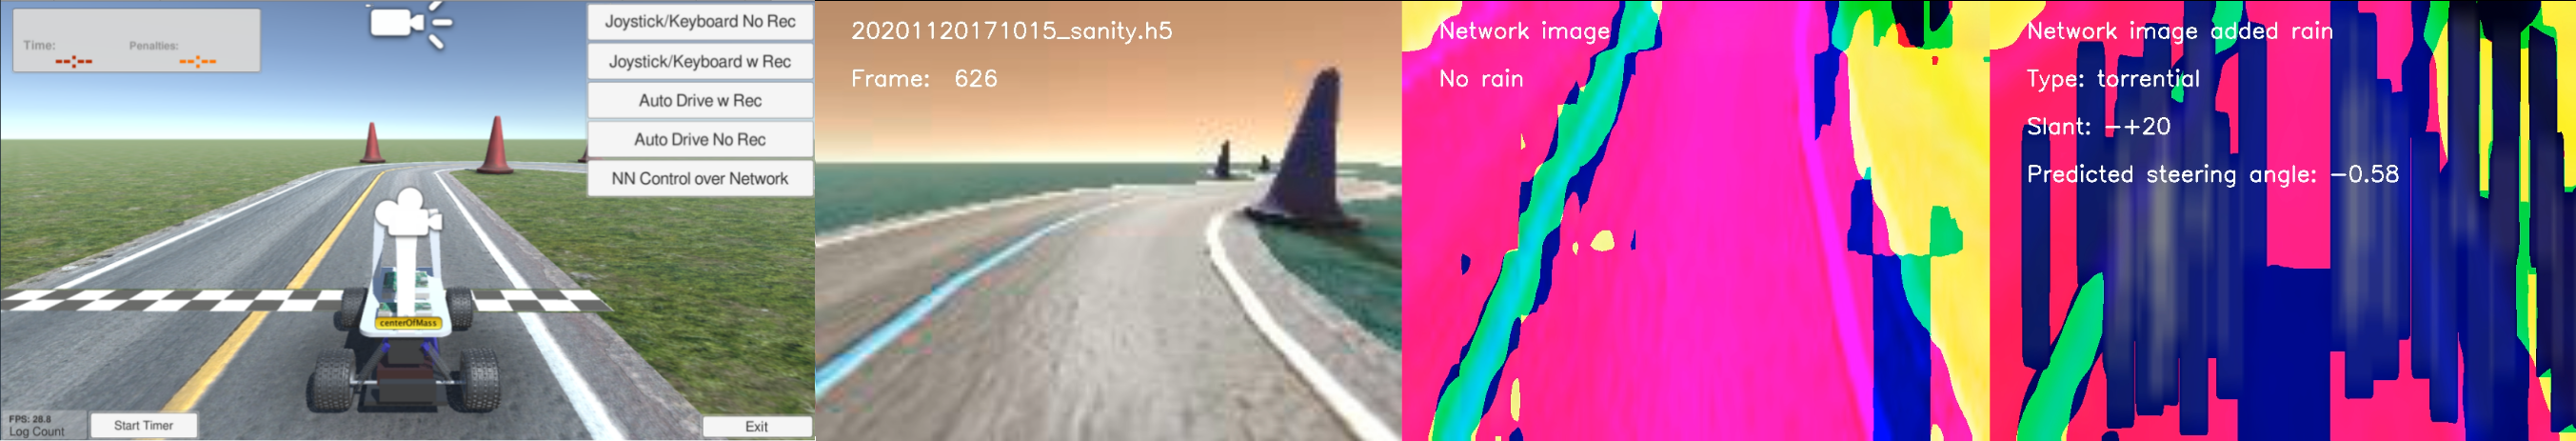
\includegraphics[width=0.99\textwidth]{Figures/Methods/UdacitySdSandboxSim.png}
\caption{Left to right, the Unity based Udacity/SDSandbox self-driving simulator desktop app, a frame capture from the simulated vehicle's front facing camera, the same image in YUV space, the image with added rain-like noisy.}
\label{fig:UdacitySdSandboxSim}
\end{figure}

Convolutional Neural Network geometries were compared.
By comparing the two best-performing CNNs, a narrow convolution model proved more robust to noise, maintaining driving performance at high noise/rain levels where the wider convolution model drove off the track. This demonstrated that network architecture is important for minimizing performance degradation under adverse conditions.
The general conclusion established that rain-like image noise does affect self-driving CNN performance, but the core safety hypothesis regarding distance metrics to quantify safety, certainty, and reliability had not yet been considered at this stage.
To "transform regression problems into multi-class classification problems" was suggested as future work, which became key in this work. 

\textbf{PhD Launch}

The PhD was funded through ICRI-SAVe, the Intel Collaborative Research Institute on Safe Automated Vehicles, which sponsored four PhD studentships focused on practical innovations advancing the state of the art, security and resilience of real-world autonomous systems. The research topic "Autonomous Systems Safety" was set, aiming at studying safe operational constraints for autonomous systems.
The distance metrics hypothesis emerged from my work with Zivid, a Norwegian manufacturer of industrial 3D depth cameras used in robotics. After approaching multiple companies seeking practical machine learning use cases for my MSc research: pitching machine learning data analytics insights to a medical equipment and a home energy metering start-ups, predictive maintenance to a medium size elevator door maintenance company and a fire suppression and detection multinational, and finally computer vision added capabilities to Zivid's camera, I got nowhere and went back to simulating autonomous vehicles in Unity. A few weeks from deadline submission of my MSc thesis, Zivid contacted me about a recent publication from \cite{sajjan2019cleargrasp3dshapeestimation} "ClearGrasp: 3D Shape Estimation of Transparent Objects for Manipulation." The challenge involved using Zivid's industrial-grade depth camera to detect transparent objects — difficult for depth cameras that rely on reflected light, as transparent objects partially refract light.
I successfully reproduced Sajjan et al.'s transparent object detection results by scaling the Zivid camera's output range to match the expected range of the Intel RealSense camera used in the original study (Figure \ref{fig:cleargrasp-D415-Zivid-pipeline-2rows}). Although Zivid ultimately deemed the resulting precision insufficient for their purposes, the experience demonstrated practical examples of data distribution shift in real-world systems, and possible solutions.

\begin{figure}[h]
\centering
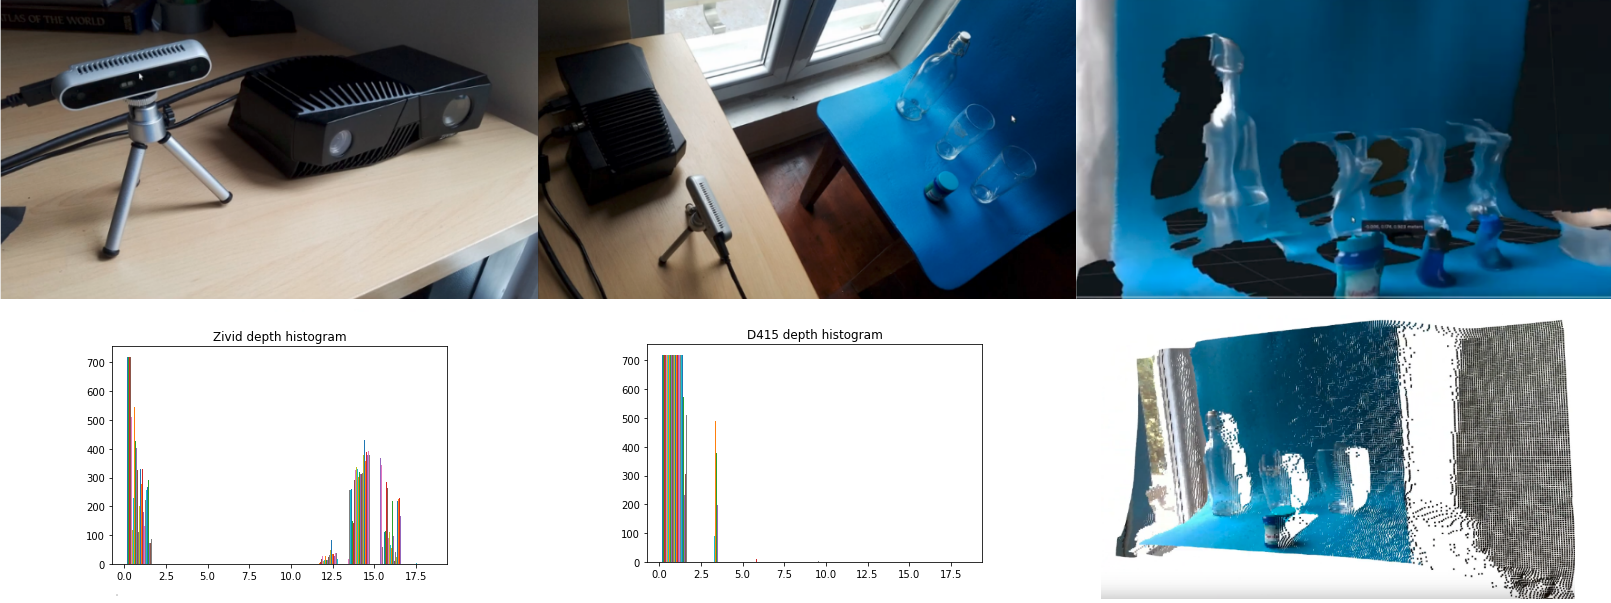
\includegraphics[width=0.99\textwidth]{Figures/Methods/cleargrasp-D415-Zivid-pipeline-2rows.png}
\caption{Top row, left to right, left: a Intel Intellisense D415 consumer grade depth camera used by \cite{sajjan2019cleargrasp3dshapeestimation}, next to a Zivid 2 industrial grade depth camera, middle: experimental setup with both Intellisense and Zivid 3D cameras facing transparent objects and right: the distorted transparent objects as displayed on the Zivid Studio camera processing desktop software \href{https://www.youtube.com/watch?v=eltQ_hvpcFs}{(video)}. Bottom row, left: the Zivid depth histogram (obtained from a point cloud object) captured in the ClearGrasp pipeline, middle: the D415 depth histogram capture at the same point and right: the Zivid image with correctly rendered surfaces once the depth distribution was scaled and made to conform to the D415 depth distribution.}
\label{fig:cleargrasp-D415-Zivid-pipeline-2rows}
\end{figure}

During an early supervisory meeting, upon reviewing the Zivid results, my supervisor, Professor Artur d'Avila Garcez - familiar with noisy data scenarios from the MSc work - suggested that out-of-distribution data detection could be a promising research avenue. Literature review identified Bhattacharyya Distance, Histogram Intersection, and KL Divergence as candidate metrics for measuring distances between original images and noise-corrupted versions, establishing the foundation for the distance-based safety assessment approach.

\textbf{The Criticism}

The first attempt to publish the idea of a safety distance metric was rejected on grounds that 1. Bhattacharyya Distance, Histogram Intersection, and KL Divergence were fragile because they operated on pixel intensities. The approach computed distances between original images from the front-facing simulated vehicle camera and the same images with added noise, but this pixel-level comparison would likely fail to capture environmental context relevant to vehicle safety, 2. the use of a non-standard (Unity simulator) dataset was noted and 3. the simulation (provided by the Unity simulator) was not realistic enough.

\begin{figure}[h]
\centering
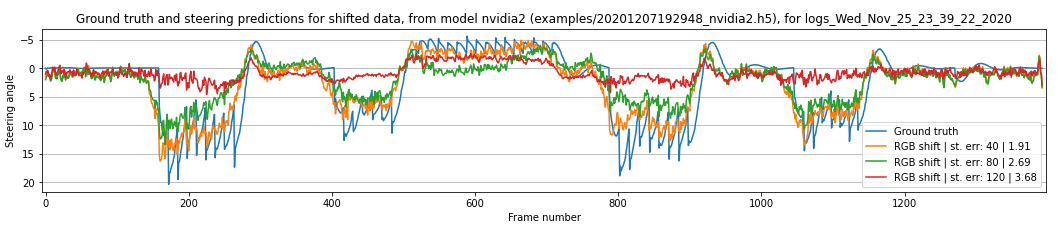
\includegraphics[width=0.99\textwidth]{Figures/Methods/dataShiftedSteeringPredictions-p40p80p120.png}
\caption{A 1.4k frame sequence capture with ground truth steering in blue, and the same data predicted with 40, 80 and 120 RGB shifts, that is the values added to individual pixels, and a result the image becoming progressively brighter (in practice the green plots would already indicate enough understeering that the vehicle would drive off the road) until saturation (red) where the models fails to predict and the vehicle is steering almost straight.}
\label{fig:dataShiftedSteeringPredictions-p40p80p120}
\end{figure}

This feedback led to a 2-year period pivot into studying the effect of noise on the standard CIFAR-10 and MNIST datasets, and to work out potential metrics to measure the level of separation between original and noise images, and the impact on neural network predictive accuracy, and becoming familiar with the CARLA ("Cars learning out to drive") simulator.

\textbf{The Pivot}

To address the use on non-standard datasets, CIFAR-10 and MNIST were studied. A pre-trained ViT \cite{google2021vitbasepatch16224} was fine-tuned on CIFAR-10, obtaining >99\% accuracy, while a CNN was trained to classify MNIST with >99\% accuracy. Then 12 different types of perturbation were applied including Gaussian Noise, Snow, Frost, and Fog. Through trial and error, function parameters were adjusted such that accuracy dropped from near 100\% to 50\% as noise intensity increased from 1 to 10, creating a linear accuracy degradation. This systematic approach generated 12 perturbation types × 10 noise levels, resulting in a 1.2M image dataset, the perturbed MNIST or the PMNIST dataset for short, for validating studying controlled network accuracy degradation.

\textbf{The Breakthrough}

The question remained, what distance metric to use between original and perturbed image. Artur suggested exploring clustering approaches, but the question of what attributes to use was pondered upon for weeks and months of PhD research darkness. The breakthrough came from a conversation with a fellow PhD research student Kaleem Peeroo, one of the co-authors in my first accepted paper (\cite{sikar2024misclassificationlikelihoodmatrixclasses}) about the softmax output layer — how it contained rich statistical information that was discarded when only the highest score was used for classification. This observation led to the realization that the softmax outputs themselves could serve as the feature space for clustering, then leading to distance metrics.

An algorithm was developed that combined supervised and unsupervised learning: K-means clustering was applied to the softmax outputs, with centroids initialized using the average softmax output for all correctly classified predictions from the original MNIST training dataset. This initialization proved effective—the algorithm converged quickly and centroids moved minimally from their starting positions. Notably, class centroids that moved most corresponded to classes with lower accuracy e.g. 8, while those that moved least had the highest accuracy e.g. 1.
The unsupervised clustering showed high fidelity to the supervised predictions: from 59,000+ predictions, all but 2 images were assigned to the same class cluster as their predicted class. With established centroids, individual softmax outputs could be positioned in the high dimensional space, enabling measurement of distances to both true and predicted class centroids.

With class centroids as anchors, statistics could be computed on the distance from predictions to their true class labels. The key insight was studying how far incorrect predictions were from their true class centroids in the cluster space. By analyzing thresholds at different distances (e.g., 0.5, 0.4, 0.3 units from the class centroid), it became possible to predict expected accuracy levels (Figure \ref{fig:MNIST_TRAINING_DATASET_ACC_RATIO_VS_THRESHOLD}). This established the fundamental relationship between distance-to-centroid and prediction reliability—noting that in the probability-constrained n-1 dimensional simplex, the maximum distance between any two vertices is square root 2.

\begin{figure}[ht!]
    \centering
    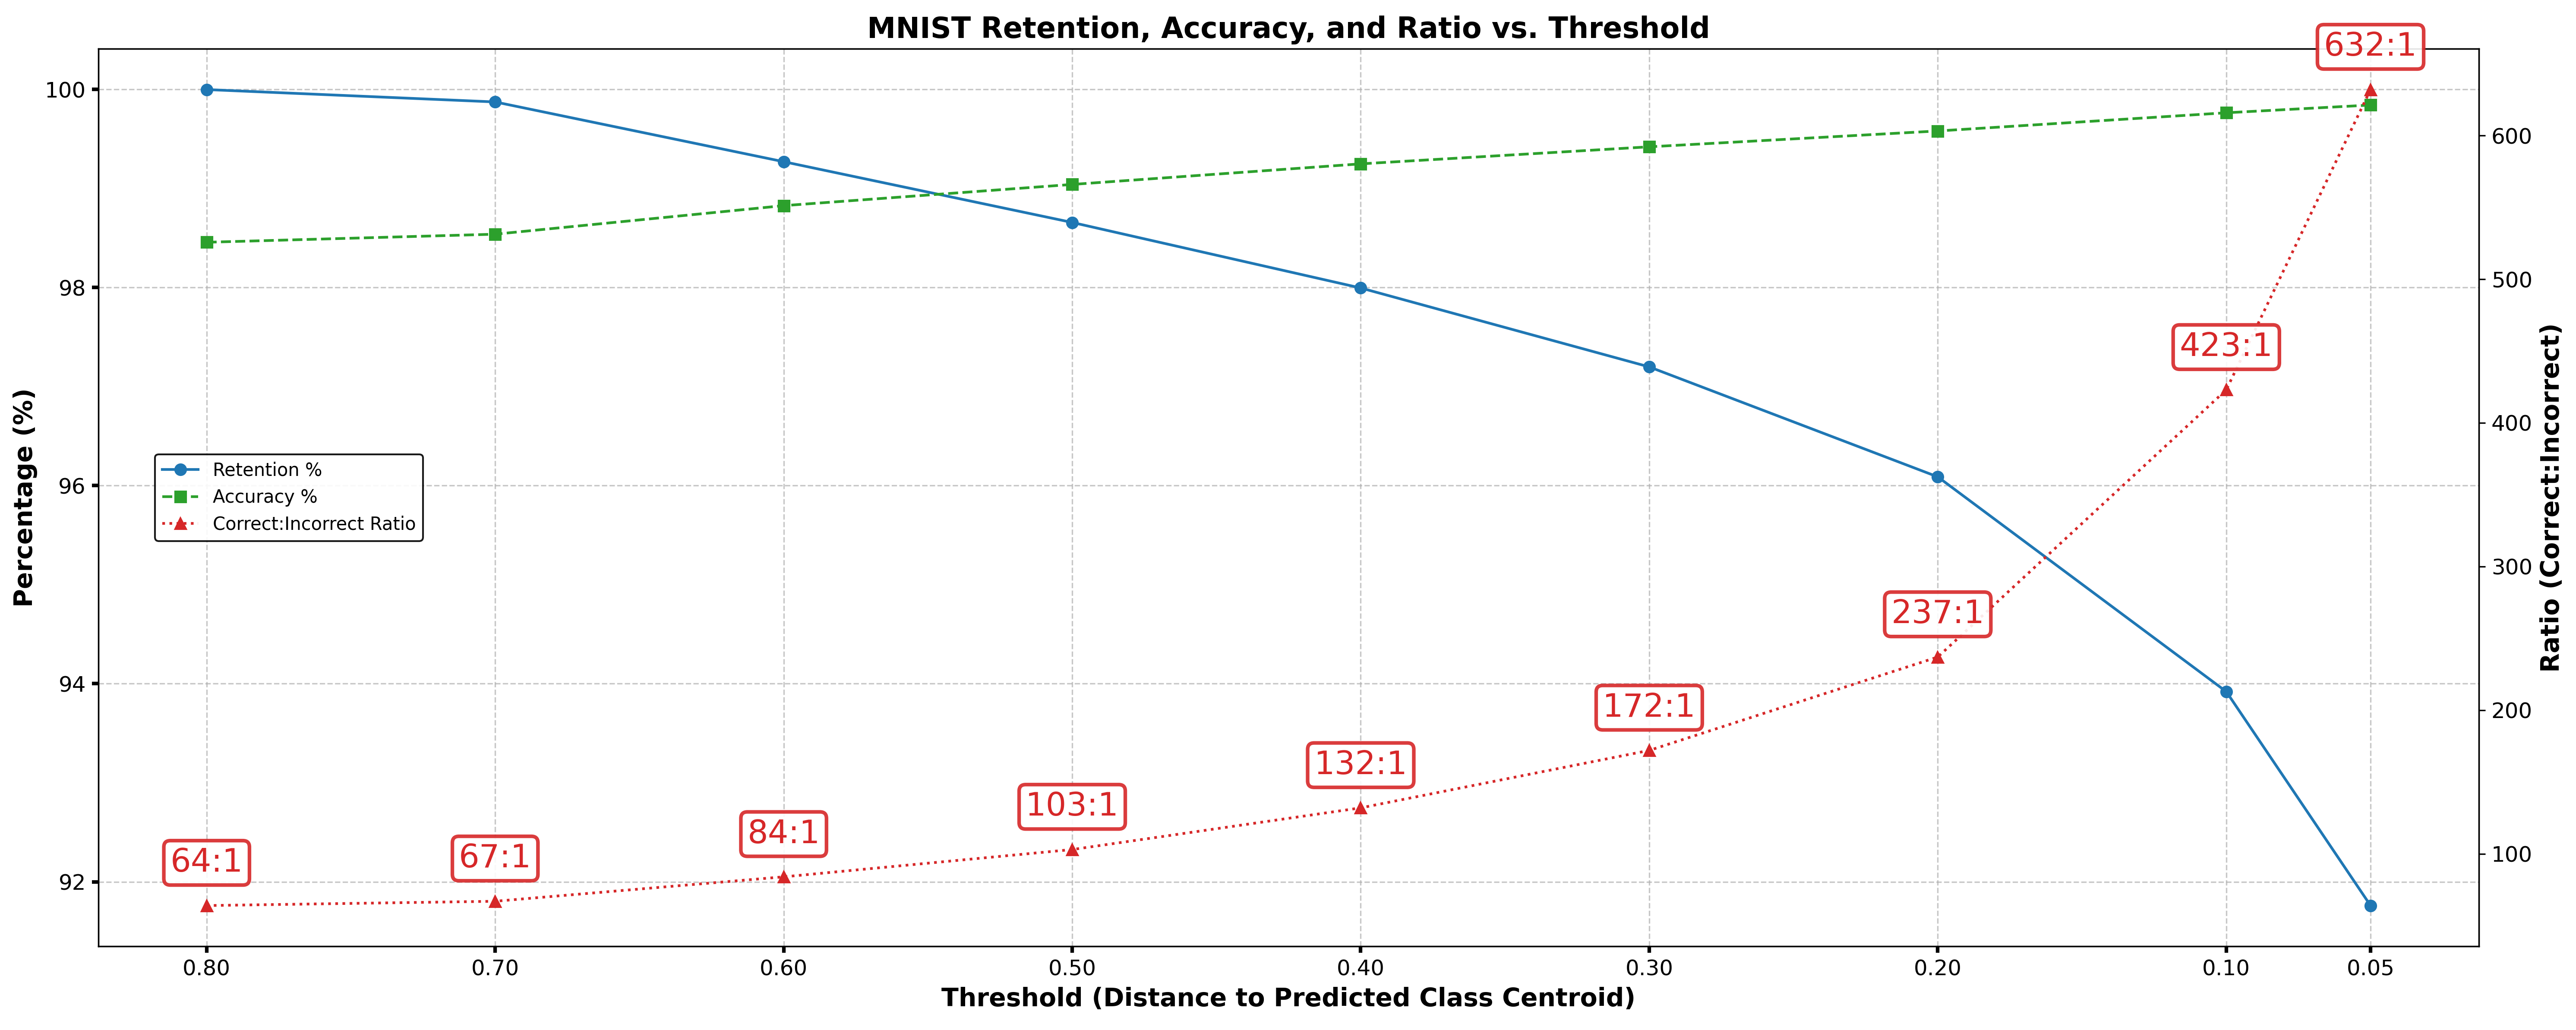
\includegraphics[width=0.99\columnwidth]{Figures/Methods/mnist_retention_accuracy_ratio_vs_threshold.png}
    \caption{A plot from the paper "Explorations of the Softmax Space: Knowing When The Network Doesn't Know" (\cite{sikar2025explorationssoftmaxspaceknowing}) showing the effect of lowering thresholds in a high dimensional softmax space for MNIST classifications, where, as the x axis threshold (distance to class centroid) decreases, the retention (blue plot - ratio of "accepted" predictions) decreases, while the accuracy (green plot) for the remaining predictions below threshold increases, while the ratio of correct:incorrect predictions below threshold increases.}
\label{fig:MNIST_TRAINING_DATASET_ACC_RATIO_VS_THRESHOLD}
\end{figure}

\textbf{Scaling Up}

Following a presentation of the intermediate results, Professor Lorenzo Stringini from the Centre for Software Reliability commented via email "- interesting to give an example of application-specific measure of actual effect of accuracy ... e.g. how often the car leaves the road (or if that is rare enough, then also how shaky the ride is, etc)", basically, inquiring about the practical application of the clustering work to autonomous systems. This challenge eventually provided the connection to an observation in the MSc dissertation's future work section, which proposed to: "transform regression problems into multi-class classification problems to make optimal use of (...) networks. This could be attained by quantizing and binning the outputs, subject to the quantized values having acceptable steering precision."
This regression-into-classification transformation would enable the methodology developed for the CIFAR-10 and MNIST datasets to be applied directly to autonomous vehicle datasets and steering angle predictions. The CARLA simulator providing the means of 1. capturing labeled datasets and 2. allowing the distance-to-centroid methodology to assess the safety of autonomous vehicle in real-time.

\textbf{The Safety Discovery}

The methodology was implemented using the CARLA simulator by first replicating the Unity simulator results. CNN and ViT networks were trained for steering angle prediction using front-facing camera images, successfully navigating a figure-of-eight dual motorway without lane invasions. These regression models were then converted to classifiers by changing the output from continuous steering angles to discrete bins (3, 5, or 15 classes).
This generated 12 models: 2 architectures (CNN, ViT) × 2 datasets (unbalanced, balanced) × 3 bin configurations. The three best-performing models were selected: CNN 5-bin on unbalanced data, ViT 5-bin, and ViT 3-bin with highest overall accuracy.
Lane invasion was defined as vehicle deviation >0.85 units from the path (approximately half the vehicle width into the adjacent lane). Progressive noise testing revealed that increasing noise levels moved predictions further from centroids. Average softmax output distances to centroids showed that below certain distance values, no lane invasions occurred while lane invasions were observed when a number of consecutive predictions were above threshold, that is the distance to centroid could be used as a operational safety limit proxy, determining when the predictions were and were not safe to use. Figure \ref{fig:PracticalApplicationAVReturnVehicleControlToHuman} shows softmax output patterns for correct predictions on the left, incorrect predictions in the middle, and the simulation, where a lane invasion occurs, on the right, where the model is steering by a ViT trained on a 5 bin unbalanced dataset subject to 60\% pepper noise (\href{https://www.youtube.com/watch?v=OyENq7Xe88Q}{video})

\begin{figure}[ht!]
    \centering
    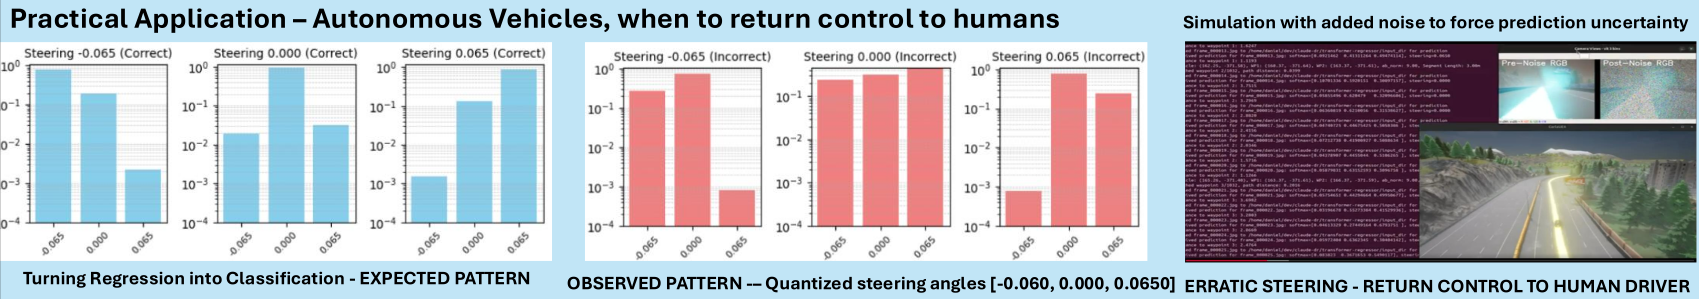
\includegraphics[width=0.99\columnwidth]{Figures/Methods/PracticalApplicationAVReturnVehicleControlToHuman.png}
    \caption{From left to right, left: average softmax outputs for correctly predicted steering angles (-0.065/left, 0.000/Straight and 0.065/Right), middle: average softmax outputs for incorrectly predicted steering angles and right: Simulations showing debug information, softmax output and distance to next path waypoint, the simulator, the image captured by vehicle camera and the same image subject to noise.}
\label{fig:PracticalApplicationAVReturnVehicleControlToHuman}
\end{figure}

This established the core safety principle: when average softmax output distances to centroids equal or exceed the threshold, the vehicle is no longer safe for autonomous operation. Analysis of the 30, 20, and 10 frame predictions preceding lane invasions showed no significant distance spikes, suggesting safety decisions could be made immediately i.e. within the first second of operation without requiring trend analysis. These findings are yet to be published.

\textbf{Advanced Exploration: VLM/MLLM Experiments}

The PhD research period (2021-2025) coincided with rapid development of Large Language Models with applications for scene understanding expanding into computer vision and robotics. Since automated vehicle steering is primarily a computer vision problem, it was logical to explore Vision Language Models/Multimodal Large Language Models (VLM/MLLM)—terms used interchangeably here as only the vision component was relevant.
The approach leveraged the models' ability to be prompted with an image and query, while a label validated predictions. The same images used to train quantized-steering CNN and ViT models were provided to VLM/MLLM systems with queries about steering direction (left, straight, or right). A series of zero-shot tests on the CIFAR-10 dataset, that is an image plus query presented to a model for prediction, where the model has not been trained on the dataset or presented an example, before progressing to steering predictions. The models used for autonomous driving were deepseek-vl-1.3b-chat (\cite{zeng2024deepseek}) and Qwen2-VL-2B-Instruct (\cite{bai2023qwen}), while Llama-3.2-11B-Vision-Instruct (\cite{meta2024llama3vision}) was used for CIFAR-10 inference. It was noted that the models, from the early CNN (200k parameters) and ViT (85M parameters) to the Vision Language Models presenting  1.3B, 2B and 11B parameters respectively increase significantly in size where the CNN runs on CPU memory, while the ViT begins to struggle and the Vision Language Models require GPU cards.
Limitations were discovered in scene understanding - the vision language models could correctly identify if a segmented lane was to the left of to the right of the vehicle, but not (in both deepseek and qwen cases) when the vehicle was directly above the segmented lane) that led to continuous lane invasions, although both models managed to complete the figure-8 circuit. The poor performance suggested that fine-tuning might lead to the precision required for safe autonomous vehicle control.
The findings relate to the distance-to-centroid methodology because VLM/MLLM models also produce softmax outputs, with prompt-dependant (i.e. constraining the reply to specific words) probability mass concentrated on the words "Left," "Straight," and "Right." This connection suggests potential future work applying the same distance-to-class centroid techniques to LLM predictions. When the realisation came, time for experiments ran out, leaving the LLM softmax space analysis as future work.

\textbf{Technical Challenges}

The research involved models of varying complexity: CNN (200k parameters), ViT (85M parameters), and VLM/MLLM (up to 2B parameters). Multiple technical challenges emerged across different scales.
Vision Transformer Training Difficulties: The 85M parameter ViT, pre-trained on ImageNet (\cite{ImageNetDeng2009}) and fine-tuned on CIFAR-10 in this study, proved extremely robust to noise, preventing achievement of the linear accuracy degradation obtained with CNN models on MNIST. Additionally, training ViT from scratch presented challenges. While pre-trained ViT (on ImageNet) achieved >99\% accuracy on CIFAR-10, training from scratch yielded maximum 89\% accuracy despite extensive experimentation with network capacity (0.5M to 100M parameters), architecture modifications, patch sizes, attention heads, and training epochs. Extended training periods hoping for "grokking" (sudden accuracy increases) proved unsuccessful. One VLM/MLLM model was used to predict CIFAR-10 never reaching 90\% accuracy, suggesting that fine-tuning would also be required to match CNN and pre-trained and fine-tuned ViT performance levels.

Lane Segmentation Workarounds: There is extensive literature on image segmentation, including lane segmentation applied to self-driving/autonomous vehicles. The CARLA simulator does provide lane segmentation that cannot isolate individual lanes, contrasting with Unity's continuous lane markings that was then hypothesised to have enabled earlier success. The workaround involved using waypoints and connecting lines to segment lanes. This is an artifact of the simulator and would not be reproducible in real life. Once clear road segmentation was achieved, CNN and ViT regressor models trained successfully, and classifier models followed, followed again the VLM/MLLM models, as the training datasets were produced.

Hardware Constraints: Local inference with deepseek-vl-1.3b-chat required upgrading from NVIDIA GeForce GTX 1060 6GB to RTX 3060 12GB to run CARLA simulator and inference concurrently. Qwen2-VL-2B-Instruct demanded even more memory, necessitating remote HPC GPU usage (NVIDIA A100 80GB). This setup introduced high latency that may have compromised results, requiring future work to determine VLM/MLLM model viability for real-time inference. The same constraints were observed with the Llama-3.2-11B-Vision-Instruct model used for CIFAR-10 zero-shot inference.